\begin{frame}{%
\begin{minipage}[t]{0.85\textwidth}
Hjejle
\end{minipage}%
\hfill
\begin{minipage}[t]{0.1\textwidth}
\raggedleft

\includegraphics[width=0.5cm, height=0.5cm, keepaspectratio]{Billeder/Ikoner/star.png}%
\hspace{0.2em}%

\includegraphics[width=0.5cm, height=0.5cm, keepaspectratio]{Billeder/Ikoner/star.png}
\end{minipage}%
}
\vspace{0.25em}
\begin{columns}[T]
% --- Venstre kolonne: Tekst ---
\column{0.55\textwidth}
\setlength{\parskip}{0.5em}
\small
\RaggedRight\textbf{\textit{Pluvialis apricaria}} – Mellemstor vadefugl som kan forveksles med strandhjejle\par 

\textbf{Udseende:} \\
\quad – Buttet krop, store øjne, rundt hoved og kort næb. Spraglet ryg med sort, grøn og hvide nuancer.  \par

\textbf{Levesteder:} \\
\quad – Marker og enge, primært Vestjylland

\textbf{Føde:} \\
\quad – Primært animals: orme, insekter, snegle  \par

\textbf{Udbredelse:} \\
\quad – Sjælden ynglefugl. Ses primært som trækfugl \par

\textbf{Træk/standfugl} \\
\quad – Trækfugl \par

% --- Højre kolonne: Kun ét billede (Hannen) ---
\column{0.40\textwidth}
\centering
\fbox{%
\begin{minipage}{\linewidth}
\centering
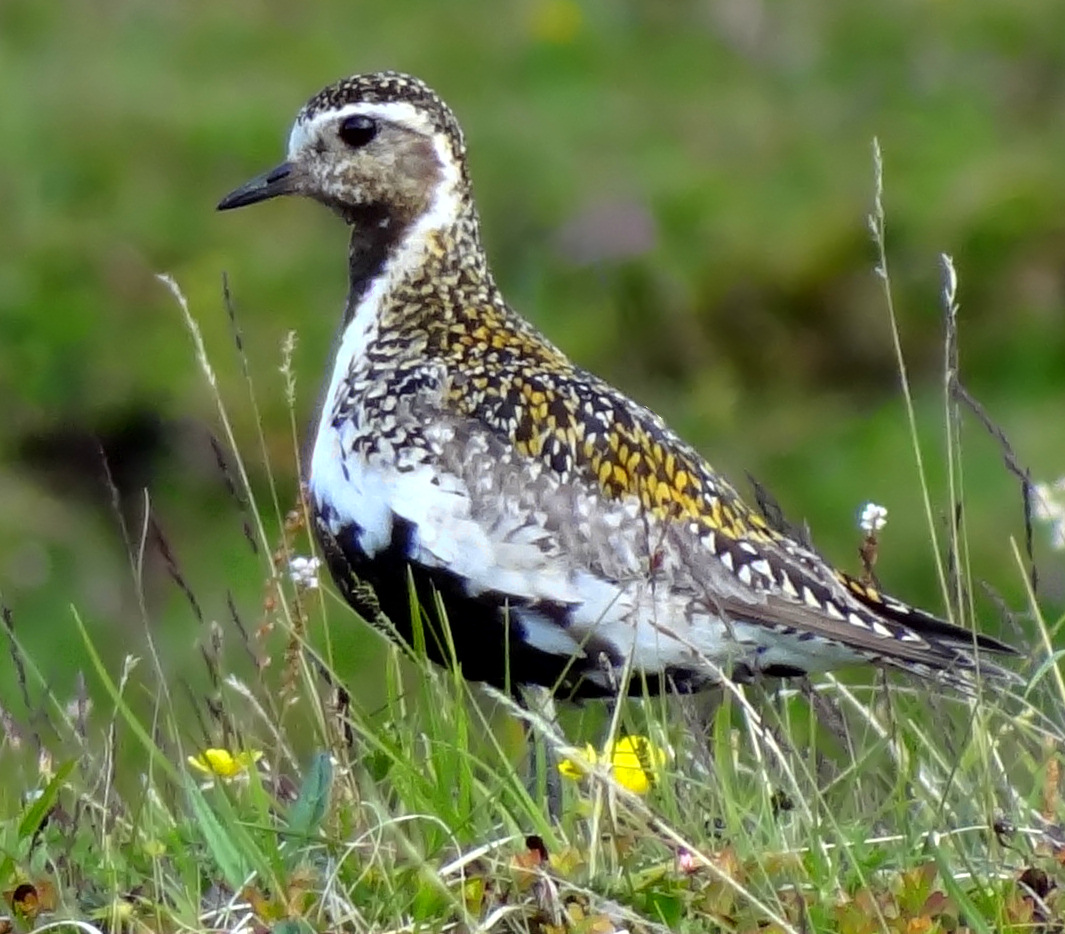
\includegraphics[width=0.8\linewidth, height=6.5cm, keepaspectratio]{Billeder/Dyr/Fugle/Vadefugle/hjejle.jpg}%
\end{minipage}
}%
\end{columns}
\end{frame}